\documentclass[a4paper, 10pt, fleqn]{article}

\usepackage[utf8]{inputenc}
\usepackage[T1]{fontenc}
\usepackage{textcomp}
\usepackage{lmodern}
\usepackage[ngerman]{babel}
\usepackage{tocbibind}
\usepackage{enumerate}
\usepackage{xcolor}
\usepackage{pdfpages}
\usepackage{amsmath}
\usepackage{graphicx}
\usepackage{geometry}
\usepackage{scrpage2}
\usepackage{lastpage}
\usepackage[hyphens]{url}
\usepackage{hyperref}
\usepackage{listings}
\usepackage{float}
\restylefloat{figure}
\lstset{language=[ansi]C++}

\newcommand{\code}[1]{\texttt{#1}}

\renewcommand*{\listoffigures}{%
  \begingroup
  \tocchapter
  \tocfile{\listfigurename}{lof}
  \endgroup
}

\geometry{left=3cm, top=3cm, bottom=3cm, right=2cm}

\hypersetup{
    colorlinks,
    linkcolor=black,
    citecolor=black,
    urlcolor=black
}

\pagestyle{scrheadings}
\ihead{PREN1 Gruppe 39}\ohead{Gesamtkonzept} 
\ifoot{\today} \ofoot{Seite \thepage\ von {\hypersetup{linkcolor=black}\pageref{LastPage}}}

% Einrücken zu Beginn von neuem Absatz unterdrücken
\setlength{\parindent}{0pt}

\begin{document}
% !TEX root = Dokumentation.tex
\begin{titlepage}   

\begin{center}
\textsc{\Large PREN Team 39}\\[0.5cm]

% Title
\newcommand{\HRule}{\rule{\linewidth}{0.5mm}}
\HRule \\[0.4cm]
{ \huge \bfseries GüselStar XXI}\\[0.4cm]
{ \LARGE \bfseries Gesamtkonzept}\\[0.4cm]
\HRule \\[1.5cm]

% Unterer Teil der Seite
{\large Horw, \today}

\begin{figure}[H]%Position festigen
\centering
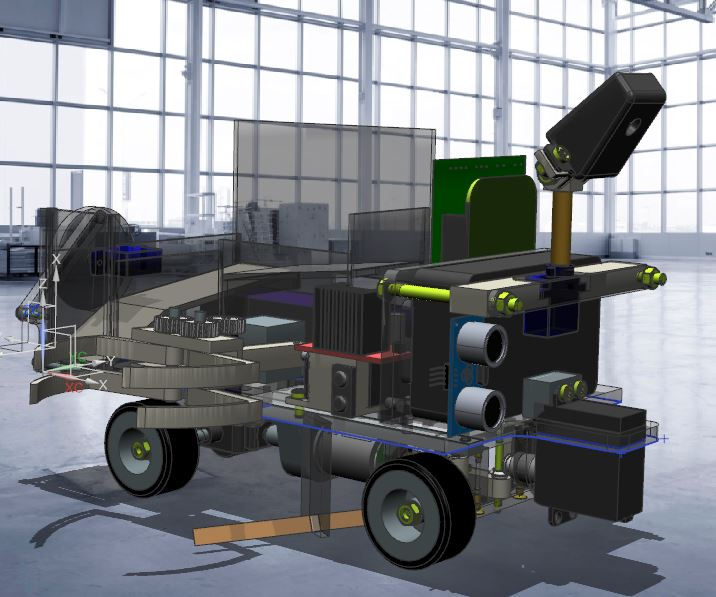
\includegraphics[width=0.7\textwidth]{03_Loesungskonzept/pictures/Tietelbild1.JPG}
\label{fig:activityRoute}
\end{figure}
% Author and supervisor
\begin{minipage}{0.4\textwidth}
\begin{flushleft} \large
\emph{Autoren:}\\
Patrizio Brantschen\\
Stefan Häfliger\\
Tobias Kreienbühl\\
Joël Meloni\\
Silvan Ritz\\
Lars Walther\\
\end{flushleft}
\end{minipage}
\hfill
\begin{minipage}{0.4\textwidth}
\begin{flushright} \large
\emph{Supervisor:} \\
Jürg Habegger
\end{flushright}
\end{minipage}
\large
\vfill
TA.BA\_PREN2.F1601 \\
Hochschule Luzern Technik \& Architektur

\end{center}

\end{titlepage}
\tableofcontents
\clearpage
\newpage
\section{Systemübersicht}
Aufgabe der UART Schnittstelle ist es, die Kommunikation zwischen Minicomputer und Mikrocontroller sicherzustellen. Dazu gehören folgende Aufgaben
\begin{itemize}
\item Austausch der Sensorwerte für die Regelkreise.
\item Definierte Kommandos um die Aktoren anzusteuern.
\end{itemize}
\section{Architektur und Designentscheide}
Um den Datenfluss einfach zu halten, werden Sensorwerte periodisch vom Freedom Board an das Raspberry Pi übertragen. Die Klasse \code{UARTReciever} ist entsprechend als Thread realisiert entschlüsselt den empfangenen String und schreibt den Wert auf entsprechende Member-Variabeln. Diese können über Funktionsgerechte Get-Methoden abgefragt werden.\\
Das Senden von Daten wird ebenfalls über Funktionsgerechte Send-Methoden von der Klasse \code{UARTSender} zur Verfügung gestellt. Entsprechend setzen diese Methoden die Ausgabestrings zusammen.
\section{Methodendefinitionen}
\subsection{UART-Methodenstrings}
\begin{tabular}{|l|l|l|l|l|} \hline
Aktor                 & Richtung    & String     & Übergabewert              & Bemerkungen \\\hline\hline
Ultraschall           & Frd => Rasp & Ul {}      & distance cm               & periodisch all 0.3s \\\hline
Flexsensor1 und ev 2  & Frd =>Rasp  & Fldist1 {} & distance mm               & periodisch all 0.2s \\\hline
StatusAuf             & Rasp=>Frd   & StA {}     & distance cm               & \\
                      & Frd=>Rasp   & StD        & abgeschlossen             & Wenn Aufladevorgang abgeschlossen \\\hline
StatusAb	              & Rasp=>Frd   & StA {}     & distance cm               & \\
                      & Frd=>Rasp   & StD        & abgeschlossen             & Wenn Entleeren abgeschlossen\\\hline
DC Motor	              & Rasp=>Frd   & DCDr{}{}   & cm pro sekunde	, hard/Soft & wenn nötig \\
Response DCDr new     & Frd=>Rasp   & DCDr{}{}   & cm pro sekunde            & wenn encoder say o \\\hline
Lenkungsservo         & Rasp=>Frd   & LeSer{}    & pbd                       & \\\hline
Kameraservo           & Rasp=>Frd   & CamPos{}   & einlenkungs pos           & \\\hline
Behälterentladung     & Rasp=>Frd   & Entl       & Entladungstrigger         & \\\hline
Debug Messages        & Frd=>Rasp   & DBG{}      & Debugmeldung              & \\\hline
NochDa                & Frd=>Rasp   & There      & Flag                      & periodisch all 0.5s \\
                      & Rasp=>Frd   & Ja         & Erhalten?                 & Wenn nein => DC stop \\\hline
Start                 & Rasp=>Frd   & StartFrd   &                           & Hochfahren und init \\
                      & Frd=>Rasp   & Ready      &                           & \\\hline
Stop	                  & Rasp=>Frd   & Stop       &                           & Programm beenden \\\hline
\end{tabular}
\end{document}